\subsection{Prototypischer Vergleich}
Im Rahmen dieser Arbeit wurde ein Prototyp der Software mit filament entwickelt.
Beide Admin-Panels koexistieren im selben Projekt.
Die neue Variante ist mit dem Präfix \enquote{/admin} in der Route aufrufbar.

Im Gegensatz zum MVP mit Nova in der Praxisprojektarbeit, handelt es sich hier allerdings um einen reinen Prototyp.
Daher liegt der Fokus nicht auf der vollständigen Umsetzung aller Features.
Dabei ist jedoch das bisherige Featureset der Sounding Console im neuen Prototyp nahezu vollständig abgebildet.

Der Fokus liegt insbesondere auf den Bereichen, die mit Nova eher problematisch waren.
So zum Beispiel die Auswertung vergangener Flüge.

\subsubsection{Positive Erfahrungen}
Die Erfahrungen mit filament waren insgesamt sehr positiv.
Auch sind kleinere Aspekte in filament schöner umgesetzt.
Ein Beispiel ist die Filterung von Tabellen.
Ausgewählte Filter werden unmittelbar oberhalb der Tabelle dargestellt (\ref{fig:active_filter_filament}).
Bei Nova versteckt sich dies erst hinter einem Klick in einem Popup (\ref{fig:active_filter_nova}).
Mit diesen Funktionen wird die Handhabung deutlich vereinfacht.

\begin{figure}[h!]
    \centering
    \caption{active filter filament}
    \label{fig:active_filter_filament}
    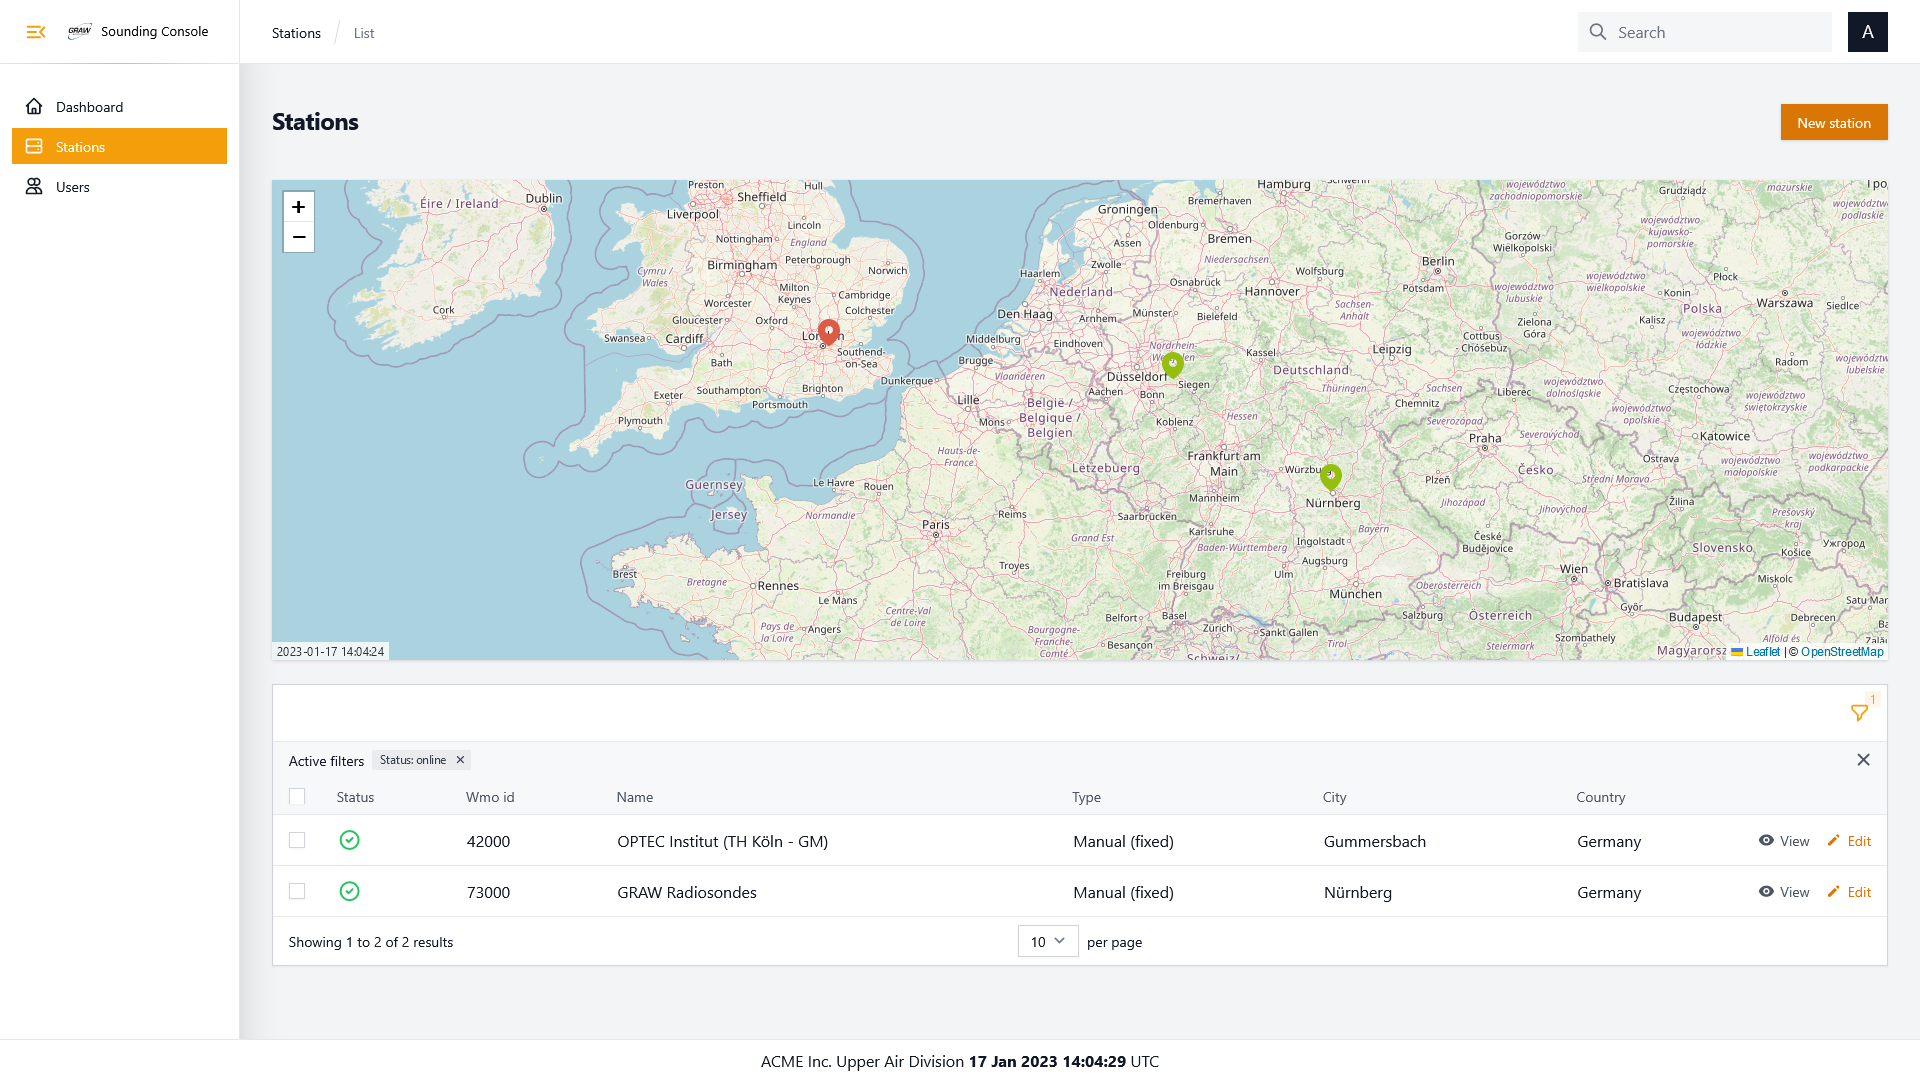
\includegraphics[scale=0.21]{assets/active_filter_filament}
\end{figure}

\begin{figure}[h!]
    \centering
    \caption{active filter nova}
    \label{fig:active_filter_nova}
    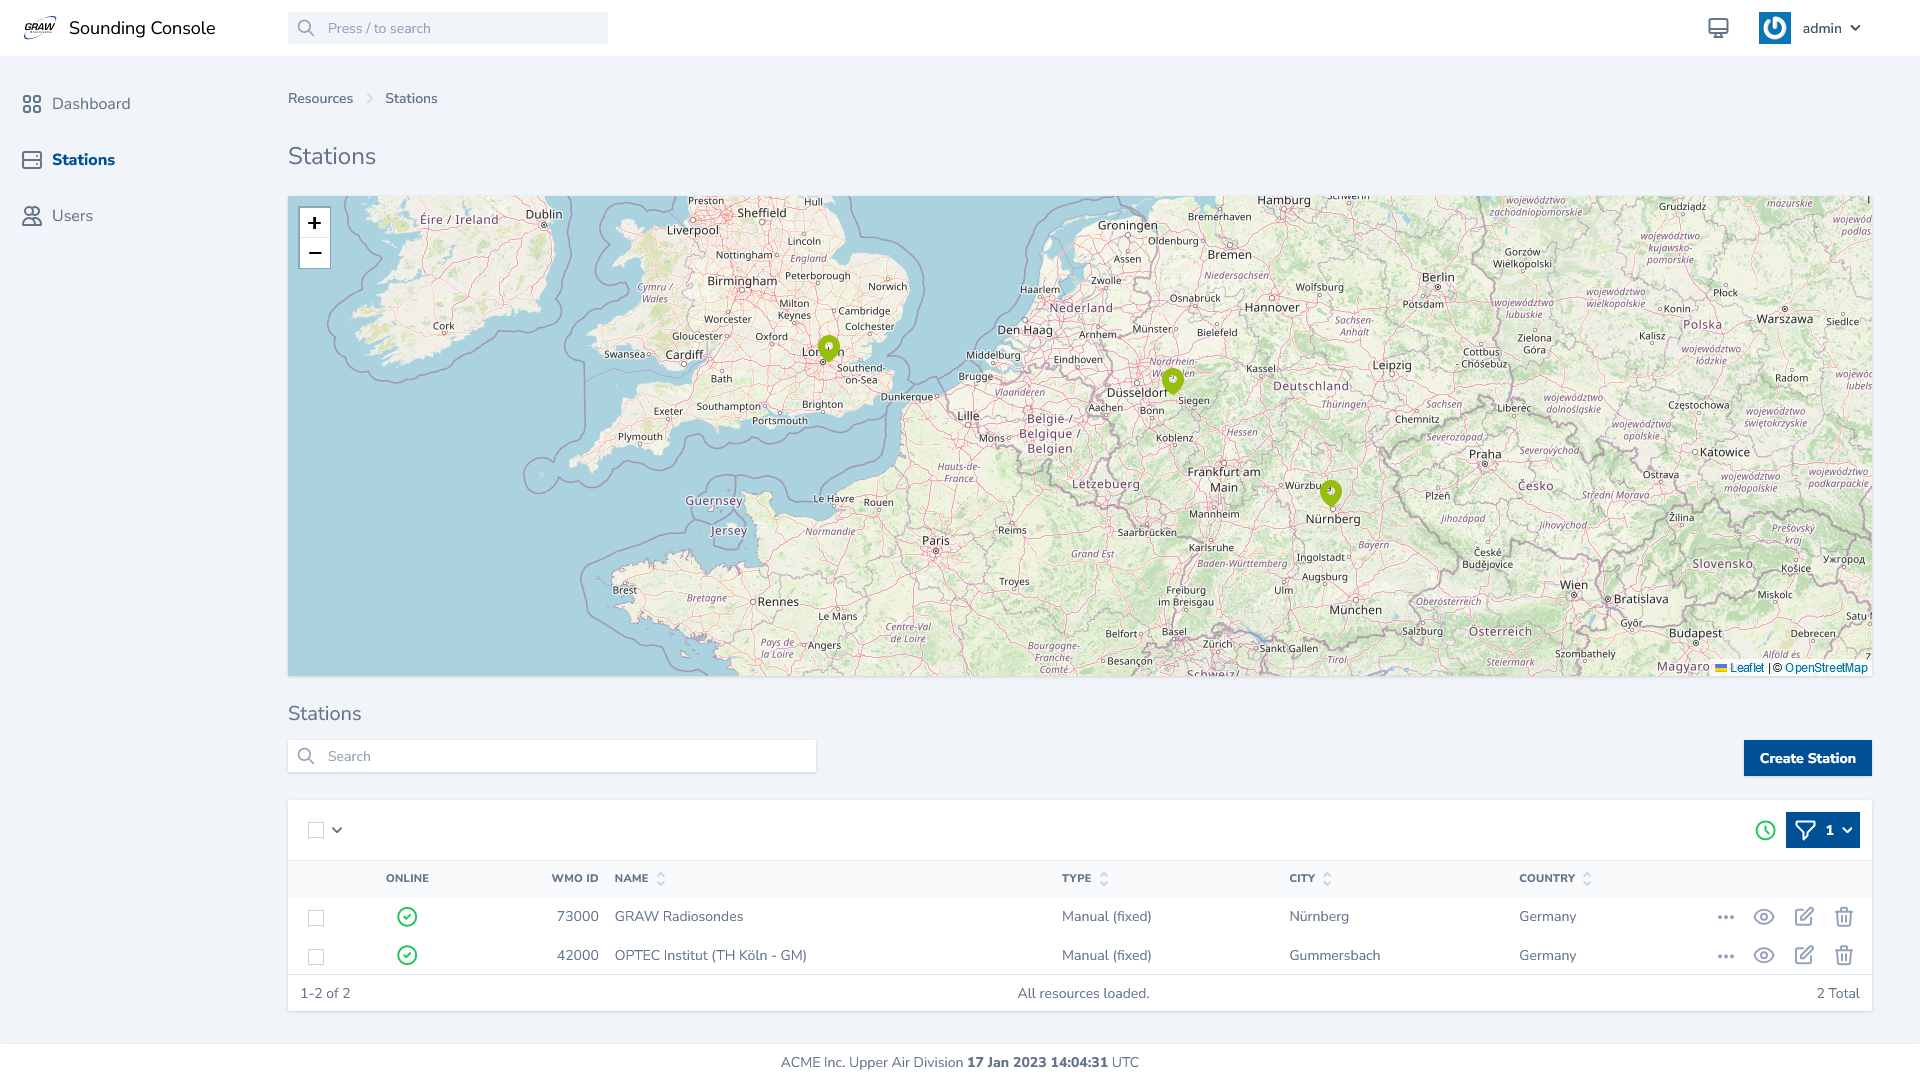
\includegraphics[scale=0.21]{assets/active_filter_nova}
\end{figure}

\newpage

\newlineparagraph{Flight View Anpassbarkeit}
Manche Ansichten benötigen weitreichende Anpassungen.
Hierzu zählt speziell der Blick auf einen vergangenen Flug.
Bei laufenden Flügen wird lediglich ein Dashboard mit aktuellen Werten und eine Karte angezeigt.
Beides passt sinnvoll oberhalb der restlichen Komponenten der Ressource, den Stammdatenfeldern und der Messwertetabelle.

Im Fall von vergangenen Flügen fällt das Dashboard weg, jedoch kommen ein Messdatendiagramm, eine Statistikübersicht und ein Skew-T-Diagramm hinzu.
Insgesamt sind das zu viele und zu große Komponenten, um diese direkt oberhalb auf der Seite zu platzieren.
Ein User müsste viel scrollen, um alles zu erfassen.
Dies wäre unübersichtlich und ineffizient.

Nova bietet kaum Möglichkeiten eine Ansicht anzupassen.
Daher war es die beste Variante, die Komponenten in Unterpunkte auszulagern (\ref{fig:finished_flight_nova}).
Nova unterstützt sogenannte Tools, welche eigenständige Seiten sind, auf denen individuelle Komponenten implementiert werden können.
Außerdem kann kontextabhängig das Menü angepasst werden.
Tests erster Nutzer zeigten allerdings, dass die entworfene Navigationsstruktur zu unübersichtlich ist.

\newpage

Filament bietet gegenüber Nova weitaus mehr Möglichkeiten, eine Ansicht individuell anzupassen.
So kann bei der vorliegenden Herausforderung eine individuelle View für den Header angegeben werden.
Diese wird oberhalb aller anderen Komponenten auf der Ansichtsseite eines Fluges gerendert.
Innerhalb dieser individuellen View kann dann eine Tab View implementiert werden, die immer nur eine größere Komponente auf einmal anzeigt (\ref{fig:finished_flight_filament}).

Die Lösung mit filament überzeugt durch eine deutlich bessere User Experience.
Die komplizierte Navigationsstruktur im Menü entfällt komplett und alles findet direkt innerhalb der Flugansicht statt.
Längeres Scrollen entfällt und die Ansicht bleibt kompakt und übersichtlich.
Filament überzeugt durch die flexible und umfangreiche Anpassbarkeit.

\begin{figure}[h!]
    \centering
    \caption{finished flight nova}
    \label{fig:finished_flight_nova}
    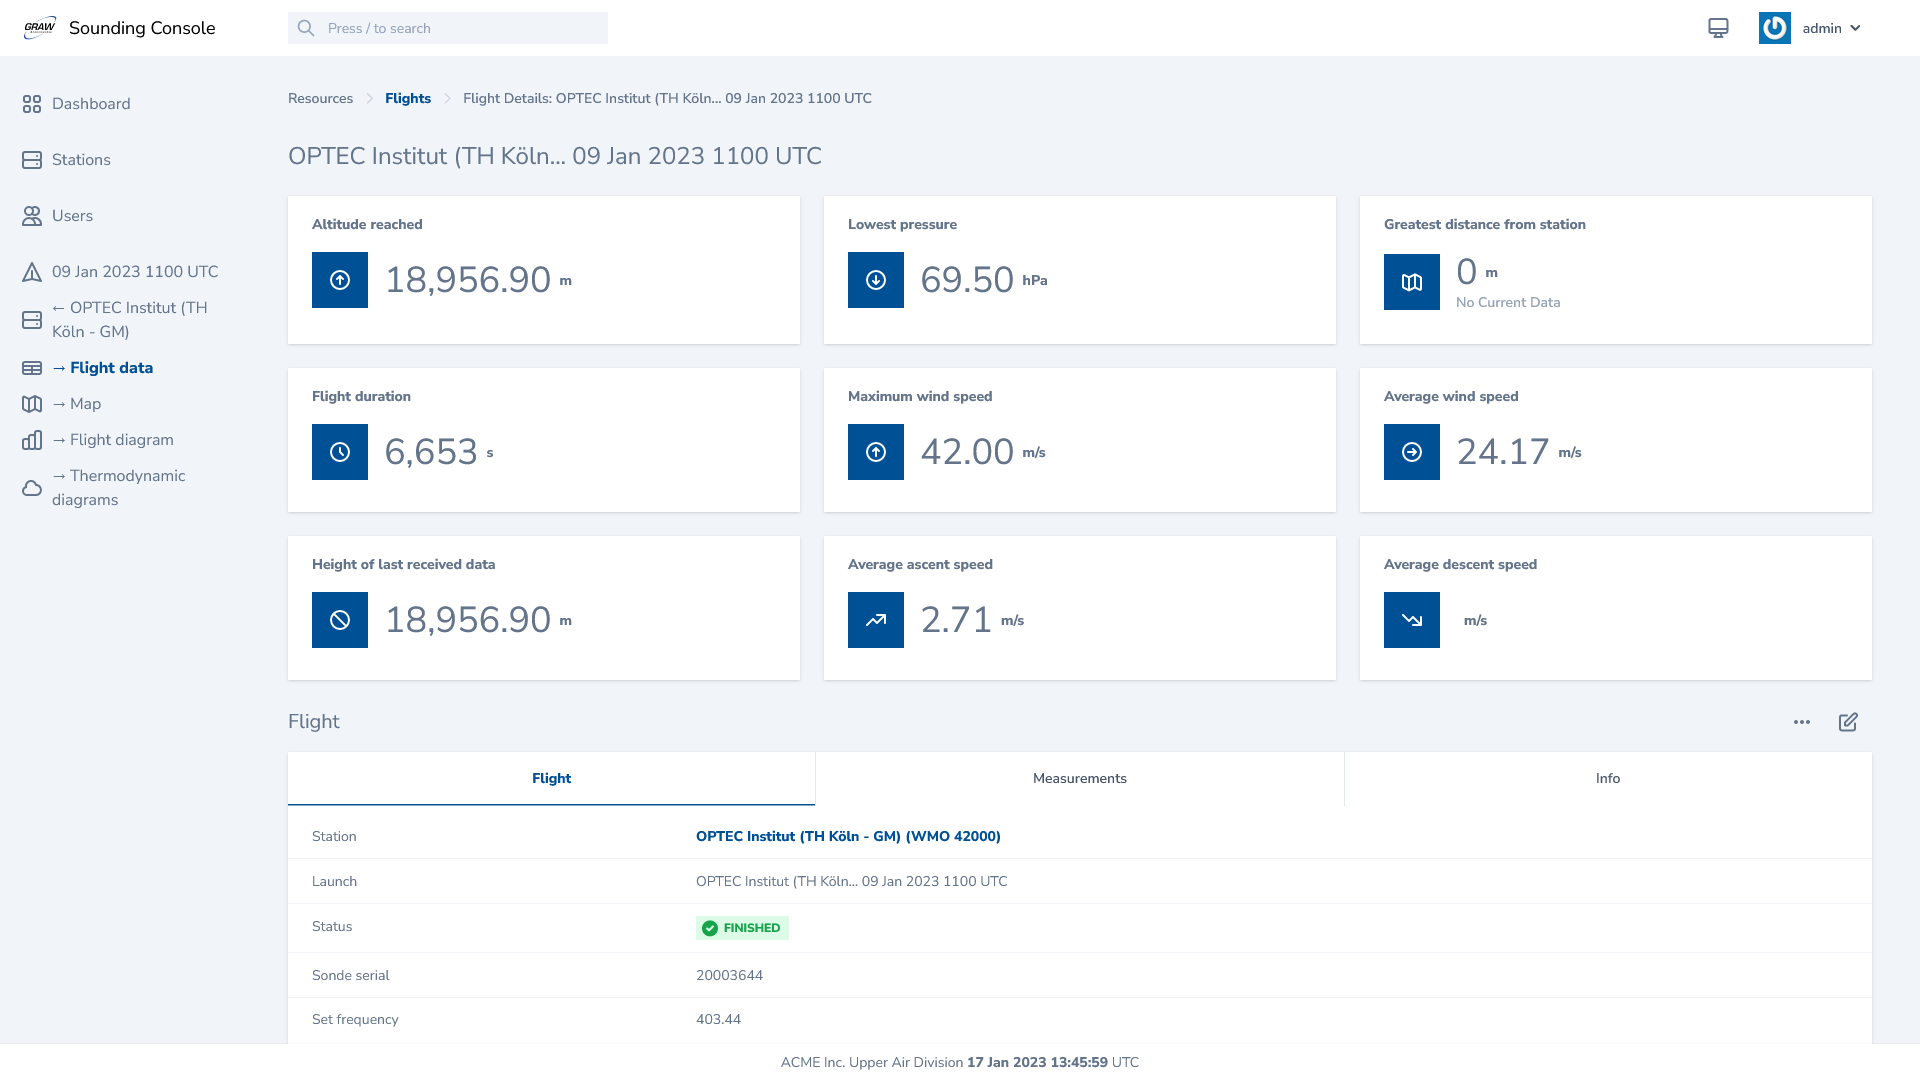
\includegraphics[scale=0.21]{assets/finished_flight_nova}
\end{figure}

\begin{figure}[h!]
    \centering
    \caption{finished flight filament}
    \label{fig:finished_flight_filament}
    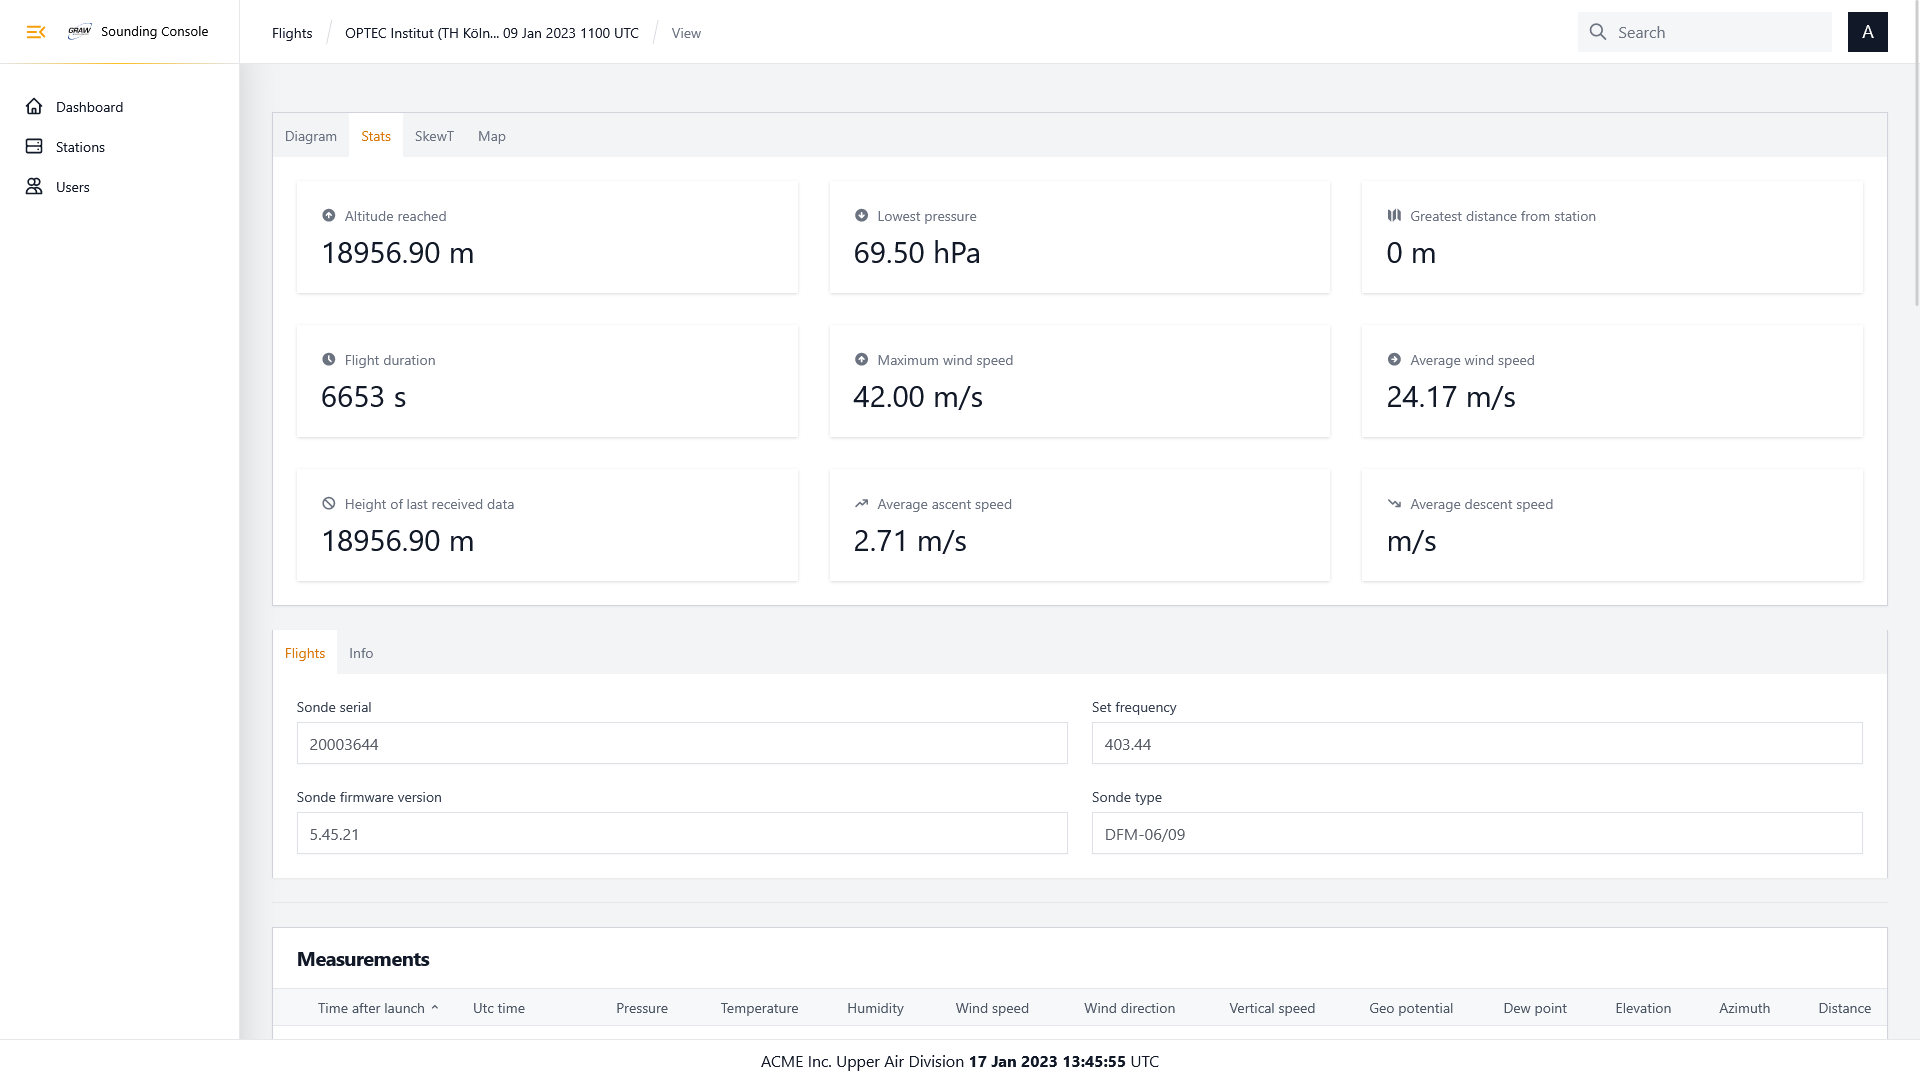
\includegraphics[scale=0.21]{assets/finished_flight_filament}
\end{figure}

\newpage

\newlineparagraph{Generelle Anpassbarkeit}
Filament punktet, durch eine generell flexiblere Anpassbarkeit.
Die Styles lassen sich besser anpassen.
Des Weiteren gibt es die Möglichkeit, an vielen Stellen individuelle Views einzuhängen.

\newlineparagraph{Ladeanimation der aktualisierenden Tabelle}
Filament zeigt keine Ladeanimation an, wenn die Tabelle neue Daten pollt.
Dadurch ist ein einfacher Vergleich der Werte möglich und die Seite springt nicht.
Die Seite springt nur, wenn neue Einträge hinzukommen.
Insgesamt ist die User Experience durch diese Animation bei filament wesentlich besser als bei Nova.

\newlineparagraph{Livewire Polling (Flight Dashboard Component)}
Filament basiert auf Livewire\cite{livewire} und somit können innerhalb einer individuellen Komponente auch Funktionen von Livewire genutzt werden.
So gibt es einen eingebauten Polling Mechanismus.
Man fügt lediglich ein Attribut zu einem HTMl Objekt hinzu und Livewire ruft dieses in einem definierbaren Intervall erneut vom Server ab.

So wurde die Implementierung des Dashboards eines laufenden Fluges vereinfacht.
Die Api und manuelles Polling mit anschließendem Austausch der Datenbasis, sodass Vue.js den Inhalt dann reaktiv updaten kann, wird nicht mehr benötigt.
Es muss nur innerhalb der Blade Komponente mit serverseitigem Code das Dashboard generiert werden und Livewire übernimmt den Rest vollautomatisch.

\newlineparagraph{Styling von Custom Components}
Nova unterstützt explizit die Verwendung der Blade Components.
So können fertige Funktionen und einheitliche Stile wiederverwendet werden.
Bei der Sounding Console werden beispielsweise Widgets als fertige Komponente geladen.

\newpage

\newlineparagraph{Infinite Loading Tables}
Filament schafft es, eine benutzbare UI mit mehreren tausenden geladenen und angezeigten Zeilen in einer Tabelle zu rendern.
Damit ist im Gegensatz zu Nova kein Infinite Load/Scroll Pattern notwendig.

Außerdem zeigt filament standardmäßig auch eine \enquote{All} Option für die Pagination an.
Dadurch kann eine zu nativen Anwendungen vergleichbare UI erstellt werden, in welcher der User durch die vollständige Tabelle scrollen kann.

\newlineparagraph{Tabellensortierung}
Ist bei filament eine Spalte als sortierbar definiert, kann für eine Ansicht ebenfalls eine Standardsortierung angegeben werden.
Dabei ist sowohl die Angabe der Spalte möglich, als auch die Sortierrichtung.
Das Problem mit Nova wird, durch diese implementierte Lösung, vollständig gelöst.

\subsubsection{Negative Erfahrungen}
Trotz aller positiven Erfahrungen gab es auch eine Hürde mit filament, welche im Folgenden erläutert ist.
Diese konnte allerdings überwunden werden, es musste lediglich auf ein neues Konzept umgestellt werden.

\newlineparagraph{Livewire Polling (Map Component)}
Das Livewire Polling Konzept ist nicht immer von Vorteil.
Bei einfachen Komponenten ist es sinnvoll, bei komplexeren Komponenten wie zum Beispiel der Karte, ist es problematisch.
Mit Nova war die Umsetzung etwas einfacher, da individuelle Nova Komponenten bereits eine geschützte HTTP Api vorbereiten, über die Updates regelmäßig abgerufen werden können.
Das Polling der gesamten Komponente ist mit filament keine Option, dennoch müssen Veränderungen erkannt und automatisch angezeigt werden.
Durch das Attribut \enquote{wire:ignore} können allerdings einzelne Bestandteile ausgenommen werden.
So wird die Karte und das dazugehörige Script nicht erneut geladen, sondern nur ein Teil, welcher bei einem Update ein Event aussendet, auf welches die Karte dann reagiert.

\newpage

\subsubsection{Implizit versus explizit}
Die prototypischen Erfahrung entsprechen denen, über die andere Entwickler\cite{reddit-laravel-nova-vs-filament} bereits berichteten.
Nova arbeitet impliziter als filament:
Felder werden an einer Stelle definiert, diese gelten dann sowohl für das Formular, als auch für die Tabelle.
Bei filament wird ein Feld mindestens an zwei Stellen definiert.

Grundsätzlich erwartet filament, dass für jede eigene Tabelle die Spalten erneut explizit definiert werden.
Dies lässt sich jedoch umgehen, indem die Tabelle aus der Ressource referenziert wird.

Die unterschiedlichen Ansätze haben ihre Vor- und Nachteile.
Der implizite Ansatz bei Nova ist schneller, insbesondere am Anfang.
Filaments explizite Definitionen benötigen initial mehr Zeit, überzeugen aber am Ende durch eine bessere und einfachere Anpassbarkeit.
Zudem ist es durchaus sinnvoll, explizit zu formulieren, wie die Felder im Formular und wie sie in Tabellen dargestellt werden sollen.
So wird verhindert, dass unerwartete Fälle eintreten, da mindestens einmal während der Entwicklung durchdacht werden muss, wie jeder Fall explizit definiert wird.
